% !TeX program = xelatex
\documentclass[a4paper,10pt]{article}

% ============================================================================
% កញ្ចប់បណ្ណាល័យ (Packages) – តាមលំនាំ NGS Preah Krasang (ls_plan.tex)
% ============================================================================
\usepackage[a4paper, left=0.95cm, right=0.95cm, top=0.85cm, bottom=0.92cm, footskip=0.52cm]{geometry}
\usepackage{amsmath}
\usepackage{unicode-math}
\usepackage{fontspec}
\usepackage{array, longtable, multirow, colortbl}
\usepackage[table]{xcolor}
\usepackage{enumitem}
\usepackage{pifont}
\usepackage{fancyhdr}
\usepackage{tikz}
\usetikzlibrary{calc, arrows.meta, angles, quotes, decorations.markings, babel}

% LaTeX 2025 + longtable v4.24 compatibility guard
\makeatletter
\let\@expl@@@mark@update@singlecol@structures@@\relax
\makeatother

% ============================================================================
% ការកំណត់ពុម្ពអក្សរ (Fonts Configuration) – តាមលំនាំស្ដង់ដារ ១០០%
% ============================================================================
% Cross-platform font path resolver (Windows local + Linux/Cloud repo fonts/)
\providecommand{\NGSFindFonts}{%
  \IfFileExists{C:/Windows/Fonts/cambria.ttc}{%
    \def\NGSSysPath{C:/Windows/Fonts/}%
    \def\NGSUserPath{C:/Users/KIT/AppData/Local/Microsoft/Windows/Fonts/}%
  }{%
    \IfFileExists{./fonts/KhmerOSsiemreap.ttf}{\def\NGSSysPath{./fonts/}\def\NGSUserPath{./fonts/}}{%
    \IfFileExists{../fonts/KhmerOSsiemreap.ttf}{\def\NGSSysPath{../fonts/}\def\NGSUserPath{../fonts/}}{%
    \IfFileExists{../../fonts/KhmerOSsiemreap.ttf}{\def\NGSSysPath{../../fonts/}\def\NGSUserPath{../../fonts/}}{%
    \IfFileExists{../../../fonts/KhmerOSsiemreap.ttf}{\def\NGSSysPath{../../../fonts/}\def\NGSUserPath{../../../fonts/}}{%
    \IfFileExists{../../../../fonts/KhmerOSsiemreap.ttf}{\def\NGSSysPath{../../../../fonts/}\def\NGSUserPath{../../../../fonts/}}{%
    \IfFileExists{../../../../../fonts/KhmerOSsiemreap.ttf}{\def\NGSSysPath{../../../../../fonts/}\def\NGSUserPath{../../../../../fonts/}}{%
    \IfFileExists{../../../../../../fonts/KhmerOSsiemreap.ttf}{\def\NGSSysPath{../../../../../../fonts/}\def\NGSUserPath{../../../../../../fonts/}}{%
      \def\NGSSysPath{../../../../../../../fonts/}\def\NGSUserPath{../../../../../../../fonts/}%
    }}}}}}}%
  }%
}
\NGSFindFonts

\setmathfont[
  Path={\NGSSysPath},
  FontIndex=1,
  Scale=1.02
]{cambria.ttc}

\defaultfontfeatures{Ligatures=TeX}

\setmainfont[
  Path={\NGSUserPath},
  Extension=.ttf,
  Script=Khmer,
  BoldFont={KhmerOSsiemreap},
  BoldFeatures={FakeBold=1.8},
  ItalicFont={KhmerOSsiemreap},
  ItalicFeatures={FakeSlant=0.25},
  BoldItalicFont={KhmerOSsiemreap},
  BoldItalicFeatures={FakeBold=1.8, FakeSlant=0.25}
]{KhmerOSsiemreap}

\newfontfamily\muol[
  Path={\NGSUserPath},
  Extension=.ttf,
  Script=Khmer
]{KhmerOSmuollight}

\newfontfamily\TimesEn[
  Path={\NGSSysPath},
  Extension=.ttf,
  Scale=1.00,
  BoldFont={timesbd},
  ItalicFont={timesi},
  BoldItalicFont={timesbi}
]{times}

\newfontfamily\NagaBold[
  Path={\NGSUserPath},
  Extension=.ttf
]{AKbalthom Naga Bold}

\newfontfamily\CalibriFont[
  Path={\NGSSysPath},
  Extension=.ttf
]{calibri}

\newfontfamily\Tacteing[
  Path={\NGSUserPath}
]{TACTENG.TTF}

\newfontfamily\CourierBullet[
  Path={\NGSSysPath},
  Extension=.ttf
]{cour}
\newcommand{\wcirc}{{\CourierBullet\fontsize{9.5pt}{11pt}\selectfont o}}

% ក្បួនកាត់ពាក្យខ្មែរ (Khmer word wrapping)
\XeTeXlinebreaklocale "km"
\XeTeXlinebreakskip = 0pt plus 1pt minus 0.1pt

% ============================================================================
% ការកំណត់ពណ៌ និងទម្រង់ទំព័រ (Colors & Page Style)
% ============================================================================
\definecolor{stepgray}{HTML}{D9D9D9}
\definecolor{headgray}{HTML}{F2F2F2}
\definecolor{boxgray}{HTML}{D9D9D9}
\definecolor{darkred}{HTML}{C00000}
\definecolor{red5e}{HTML}{FF0000}

\pagestyle{fancy}
\fancyhf{}
\renewcommand{\headrulewidth}{0pt}
\fancyfoot[R]{\CalibriFont\fontsize{11pt}{13pt}\selectfont\thepage}

\setlength{\parindent}{0pt}
\setlength{\parskip}{0pt}
\setlength{\tabcolsep}{3.8pt}

\newcolumntype{L}[1]{>{\raggedright\arraybackslash}p{#1}}

% ============================================================================
% ម៉ាក្រូជំនួយ (Helper Macros)
% ============================================================================
\newcommand{\en}[1]{{\TimesEn #1}}
\newcommand{\enbf}[1]{{\TimesEn\textbf{#1}}}
\newcommand{\unit}[1]{\,\text{\en{#1}}}
\newcommand{\fiveE}[1]{{\NagaBold\fontsize{9.5pt}{13pt}\selectfont\textcolor{red5e}{#1}}}
\newcommand{\timenote}[1]{\textcolor{darkred}{\textit{#1}}}
\newcommand{\redsub}[1]{\textcolor{darkred}{#1}}
\newcommand{\graybox}[1]{\colorbox{boxgray}{\strut\hspace{2pt}#1\hspace{2pt}}}
\newcommand{\ditem}{\tikz[baseline=-0.5ex]\fill (0,0.42ex) -- (0.42ex,0) -- (0,-0.42ex) -- (-0.42ex,0) -- cycle;\hspace{0.3em}}
\newcommand{\cnum}[1]{{\fontsize{10.5pt}{12pt}\selectfont\ding{\numexpr181+#1\relax}}\hspace{0.2em}}
\newcommand{\cfig}[1]{\par\vspace{1.2pt}{\centering #1\par}\vspace{1.2pt}}
\newcommand{\stepheader}[1]{\multicolumn{3}{|c|}{\cellcolor{stepgray}\muol #1} \\* \noalign{\hrule height 0.4pt}}
\newcommand{\tri}[1]{\ensuremath{\triangle #1}}
\newcommand{\ang}[1]{\ensuremath{\angle #1}}
\newcommand{\cg}{\ensuremath{\cong}}
\newcommand{\ncg}{\ensuremath{\not\cong}}

% រចនាប័ទ្មគូសសម្គាល់ជ្រុងស្មើគ្នា (Tick mark styles - bold B&W print safe)
\tikzset{
  tk1/.style={postaction={decorate},decoration={markings,mark=at position 0.50 with {\draw[black, line width=0.85pt](0,-0.095)--(0,0.095);}}},
  tk2/.style={postaction={decorate},decoration={markings,
    mark=at position 0.45 with {\draw[black, line width=0.85pt](0,-0.095)--(0,0.095);},
    mark=at position 0.55 with {\draw[black, line width=0.85pt](0,-0.095)--(0,0.095);}}},
  tkslash/.style={postaction={decorate},decoration={markings,mark=at position 0.50 with {\draw[black, line width=0.85pt](-0.065,-0.075)--(0.065,0.075);}}},
  hypArrow/.style={black, densely dashed, line width=0.8pt, -{Stealth[length=3.5pt]}}
}

% ម៉ាក្រូគូសប្រអប់មុំកែង 90° ត្រង់ #3 ក្នុងមុំ #2-#3-#4
\newcommand{\rightbox}[4][0.19]{%
  \draw[black, line width=0.8pt]
    ($(#3)!#1!(#2)$) -- ($($(#3)!#1!(#2)$)+($(#3)!#1!(#4)$)-(#3)$) -- ($(#3)!#1!(#4)$);
}

% ក្បាច់ក្រោមបាវចនា (Tacteing Font - Keyboard '3')
\newcommand{\khmflourish}{{\Tacteing\fontsize{36pt}{14pt}\selectfont\raisebox{-5pt}{3}}}

% ============================================================================
% ម៉ាក្រូគូសរូបធរណីមាត្រ (Monochrome B&W TikZ Figures, 100% Black Text)
% ============================================================================

% ១. កំណែកិច្ចការផ្ទះមេរៀនមុន (លំហាត់ #2 ទំ.១៦៤ & #8, #11 ទំ.១៦៥)
\newcommand{\figHWoldINEQ}{%
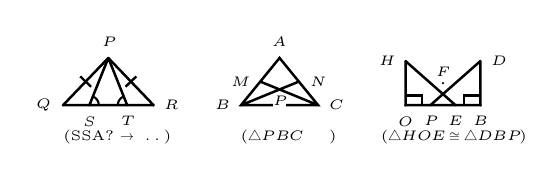
\begin{tikzpicture}[scale=0.50, every node/.style={font=\tiny, text=black}]
  % ទី២ (ទំ.១៦៤)
  \begin{scope}[shift={(-4.35,0)}]
    \coordinate (P) at (0,1.20);
    \coordinate (Q) at (-1.15,0);
    \coordinate (R) at (1.15,0);
    \coordinate (S) at (-0.48,0);
    \coordinate (T) at (0.48,0);
    \draw[black, line width=0.9pt, tk1] (P) -- (Q);
    \draw[black, line width=0.9pt, tk1] (P) -- (R);
    \draw[black, line width=0.9pt] (Q) -- (R) (P) -- (S) (P) -- (T);
    \draw[black, line width=0.75pt] ($(S)+(0:0.24)$) arc (0:68:0.24);
    \draw[black, line width=0.75pt] ($(T)+(180:0.24)$) arc (180:112:0.24);
    \fill[black] (P) circle (1.0pt) node[above=0.5pt] {$P$};
    \fill[black] (Q) circle (1.0pt) node[left=0.5pt] {$Q$};
    \fill[black] (R) circle (1.0pt) node[right=0.5pt] {$R$};
    \fill[black] (S) circle (0.9pt) node[below=0.5pt] {$S$};
    \fill[black] (T) circle (0.9pt) node[below=0.5pt] {$T$};
    \node[fill=white, inner sep=0.4pt] at (0,-0.82) {ទី២ (\en{SSA?} $\to$ ជ.ម.ជ)};
  \end{scope}
  % ទី៨ (ទំ.១៦៥)
  \begin{scope}[shift={(0.00,0)}]
    \coordinate (A) at (0,1.20);
    \coordinate (B) at (-0.98,0);
    \coordinate (C) at (0.98,0);
    \coordinate (M) at ($(A)!0.5!(B)$);
    \coordinate (N) at ($(A)!0.5!(C)$);
    \coordinate (P) at (0,0.40);
    \draw[black, line width=0.9pt] (A) -- (B) -- (C) -- cycle (B) -- (N) (C) -- (M);
    \fill[black] (A) circle (1.0pt) node[above=0.5pt] {$A$};
    \fill[black] (B) circle (1.0pt) node[left=0.5pt] {$B$};
    \fill[black] (C) circle (1.0pt) node[right=0.5pt] {$C$};
    \fill[black] (M) circle (0.9pt) node[left=0.5pt] {$M$};
    \fill[black] (N) circle (0.9pt) node[right=0.5pt] {$N$};
    \fill[black] (P) circle (0.9pt) node[below=2pt, fill=white, inner sep=0.3pt] {$P$};
    \node[fill=white, inner sep=0.4pt] at (0,-0.82) {ទី៨ ($\tri{PBC}$ សមបាទ)};
  \end{scope}
  % ទី១១ (ទំ.១៦៥)
  \begin{scope}[shift={(4.15,0)}]
    \coordinate (O) at (-0.95,0);
    \coordinate (B) at (0.95,0);
    \coordinate (P) at (-0.32,0);
    \coordinate (E) at (0.32,0);
    \coordinate (H) at (-0.95,1.12);
    \coordinate (D) at (0.95,1.12);
    \coordinate (F) at (0,0.56);
    \draw[black, line width=0.9pt] (H) -- (O) -- (B) -- (D) (H) -- (E) (D) -- (P);
    \rightbox[0.22]{H}{O}{B}
    \rightbox[0.22]{D}{B}{O}
    \fill[black] (H) circle (1.0pt) node[left=0.5pt] {$H$};
    \fill[black] (D) circle (1.0pt) node[right=0.5pt] {$D$};
    \fill[black] (O) circle (1.0pt) node[below=0.5pt] {$O$};
    \fill[black] (P) circle (0.9pt) node[below=0.5pt] {$P$};
    \fill[black] (E) circle (0.9pt) node[below=0.5pt] {$E$};
    \fill[black] (B) circle (1.0pt) node[below=0.5pt] {$B$};
    \fill[black] (F) circle (0.9pt) node[above=2pt, fill=white, inner sep=0.3pt] {$F$};
    \node[fill=white, inner sep=0.4pt] at (0,-0.82) {ទី១១ ($\tri{HOE}\cg\tri{DBP}$)};
  \end{scope}
\end{tikzpicture}}

% ២. រំលឹកមេរៀនទាក់ទង៖ មុំក្រៅ + សមបាទ + ក្បួនអក្សរទី៣ ដែលបាត់
\newcommand{\figPrereqINEQ}{%
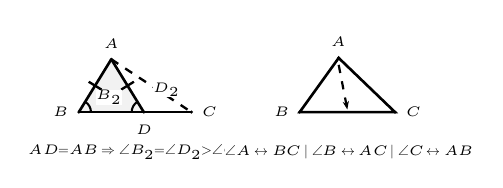
\begin{tikzpicture}[scale=0.55, every node/.style={font=\tiny, text=black}]
  % ឆ្វេង៖ មុំក្រៅ និងសមបាទ
  \begin{scope}[shift={(-2.65,0)}]
    \coordinate (B) at (-1.05,0);
    \coordinate (D) at (0.45,0);
    \coordinate (C) at (1.55,0);
    \coordinate (A) at (-0.30,1.22);
    \fill[gray!10] (A) -- (B) -- (D) -- cycle;
    \draw[black, line width=0.95pt, tk1] (A) -- (B);
    \draw[black, line width=0.95pt, tk1] (A) -- (D);
    \draw[black, line width=0.95pt] (B) -- (C);
    \draw[black, line width=0.85pt, dashed] (A) -- (C);
    \draw[black, line width=0.75pt] ($(B)+(0:0.28)$) arc (0:58:0.28);
    \draw[black, line width=0.75pt] ($(D)+(180:0.28)$) arc (180:122:0.28);
    \fill[black] (A) circle (1.1pt) node[above=0.5pt] {$A$};
    \fill[black] (B) circle (1.1pt) node[left=0.5pt] {$B$};
    \fill[black] (D) circle (1.1pt) node[below=1pt] {$D$};
    \fill[black] (C) circle (1.1pt) node[right=0.5pt] {$C$};
    \node[fill=white, inner sep=0.3pt] at (-0.35,0.34) {$B_2$};
    \node[fill=white, inner sep=0.3pt] at (0.98,0.52) {$D_2$};
    \node[fill=white, inner sep=0.4pt] at (0.20,-0.92) {$AD{=}AB \Rightarrow \ang{B_2}{=}\ang{D_2}{>}\ang{C}$};
  \end{scope}
  % ស្ដាំ៖ ក្បួនអក្សរទី៣ ដែលបាត់ក្នុង △ABC
  \begin{scope}[shift={(2.45,0)}]
    \coordinate (B) at (-1.05,0);
    \coordinate (C) at (1.15,0);
    \coordinate (A) at (-0.15,1.25);
    \draw[black, line width=0.95pt] (A) -- (B) -- (C) -- cycle;
    \draw[black, line width=0.8pt, dashed, -{Stealth[length=3pt]}] ($(A)+(0,-0.16)$) -- (0.05,0.06);
    \fill[black] (A) circle (1.1pt) node[above=0.5pt] {$A$};
    \fill[black] (B) circle (1.1pt) node[left=0.5pt] {$B$};
    \fill[black] (C) circle (1.1pt) node[right=0.5pt] {$C$};
    \node[fill=white, inner sep=0.4pt] at (0.10,-0.92) {$\ang{A}\leftrightarrow BC \;\vert\; \ang{B}\leftrightarrow AC \;\vert\; \ang{C}\leftrightarrow AB$};
  \end{scope}
\end{tikzpicture}}

% ៣. E1 Engage: ដងស្ទូច និងខ្សែរ៉កបើកមុំទ្វារទឹក (4 m & 7 m arms)
\newcommand{\figEngageINEQ}{%
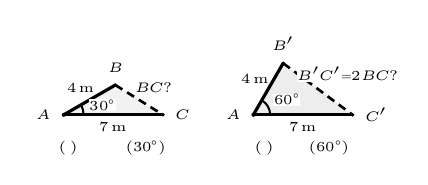
\begin{tikzpicture}[scale=0.56, every node/.style={font=\tiny, text=black}]
  % (១) មុំបើក 30°
  \begin{scope}[shift={(-2.55,0)}]
    \coordinate (A) at (0,0);
    \coordinate (C) at (2.25,0);
    \coordinate (B) at (30:1.35);
    \fill[gray!10] (A) -- (B) -- (C) -- cycle;
    \draw[black, line width=1.15pt] (A) -- (B);
    \draw[black, line width=1.15pt] (A) -- (C);
    \draw[black, line width=0.95pt, densely dashed] (B) -- (C);
    \draw[black, line width=0.75pt] (0.45,0) arc (0:30:0.45);
    \fill[black] (A) circle (1.3pt) node[left=1pt] {$A$};
    \fill[black] (B) circle (1.2pt) node[above=1pt] {$B$};
    \fill[black] (C) circle (1.2pt) node[right=1pt] {$C$};
    \node[fill=white, inner sep=0.3pt] at (0.88,0.22) {$30^\circ$};
    \node[fill=white, inner sep=0.3pt] at (0.38,0.62) {$4\unit{m}$};
    \node[fill=white, inner sep=0.3pt] at (1.12,-0.28) {$7\unit{m}$};
    \node[fill=white, inner sep=0.3pt] at (2.05,0.62) {$BC?$};
    \node[fill=white, inner sep=0.4pt] at (1.10,-0.76) {(១) មុំបើកតូច ($30^\circ$)};
  \end{scope}
  % (២) មុំបើកគុណ ២ (60°)
  \begin{scope}[shift={(1.75,0)}]
    \coordinate (A) at (0,0);
    \coordinate (Cp) at (2.25,0);
    \coordinate (Bp) at (60:1.35);
    \fill[gray!14] (A) -- (Bp) -- (Cp) -- cycle;
    \draw[black, line width=1.15pt] (A) -- (Bp);
    \draw[black, line width=1.15pt] (A) -- (Cp);
    \draw[black, line width=0.95pt, densely dashed] (Bp) -- (Cp);
    \draw[black, line width=0.75pt] (0.38,0) arc (0:60:0.38);
    \fill[black] (A) circle (1.3pt) node[left=1pt] {$A$};
    \fill[black] (Bp) circle (1.2pt) node[above=1pt] {$B'$};
    \fill[black] (Cp) circle (1.2pt) node[right=1pt] {$C'$};
    \node[fill=white, inner sep=0.3pt] at (0.76,0.34) {$60^\circ$};
    \node[fill=white, inner sep=0.3pt] at (0.04,0.82) {$4\unit{m}$};
    \node[fill=white, inner sep=0.3pt] at (1.12,-0.28) {$7\unit{m}$};
    \node[fill=white, inner sep=0.3pt] at (2.15,0.92) {$B'C'{=}2BC?$};
    \node[fill=white, inner sep=0.4pt] at (1.10,-0.76) {(២) គុណ ២ ($60^\circ$)};
  \end{scope}
\end{tikzpicture}}

% ៤. E2 Act 1: កាត់/បត់ ១:១ △ABC (AB=4.00, BC=5.50, AC=6.50 cm, AD=AB=4.00 cm)
\newcommand{\figExploreOneINEQ}{%
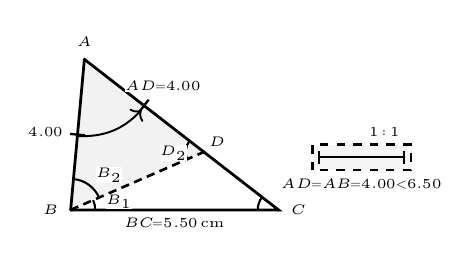
\begin{tikzpicture}[scale=0.48, every node/.style={font=\tiny, text=black}]
  % ត្រីកោណ ABC តាមសមាមាត្រពិត 1:1
  \begin{scope}[shift={(-2.65,0)}]
    \coordinate (B) at (0,0);
    \coordinate (C) at (5.50,0);
    \coordinate (A) at (0.3636,3.9834);
    \coordinate (D) at (3.5245,1.5321);
    \fill[gray!10] (A) -- (B) -- (D) -- cycle;
    \draw[black, line width=1.0pt, tk1] (A) -- (B);
    \draw[black, line width=1.0pt, tk1] (A) -- (D);
    \draw[black, line width=1.0pt] (D) -- (C) -- (B);
    \draw[black, line width=0.95pt, densely dashed] (B) -- (D);
    \draw[black, line width=0.75pt] ($(B)+(0:0.65)$) arc (0:23.5:0.65);
    \draw[black, line width=0.75pt] ($(B)+(23.5:0.82)$) arc (23.5:84.8:0.82);
    \draw[black, line width=0.75pt] ($(D)+(142.2:0.48)$) arc (142.2:203.5:0.48);
    \draw[black, line width=0.75pt] ($(C)+(142.2:0.55)$) arc (142.2:180:0.55);
    \draw[black, line width=0.7pt, ->, bend right=24] (0.20,1.95) to (1.88,2.65);
    \fill[black] (A) circle (1.3pt) node[above=1pt] {$A$};
    \fill[black] (B) circle (1.3pt) node[left=1pt] {$B$};
    \fill[black] (C) circle (1.3pt) node[right=1pt] {$C$};
    \fill[black] (D) circle (1.3pt) node[above right=1.5pt, fill=white, inner sep=0.4pt] {$D$};
    \node[fill=white, inner sep=0.4pt] at (-0.65,2.05) {$4.00$};
    \node[fill=white, inner sep=0.4pt] at (2.45,3.28) {$AD{=}4.00$};
    \node[fill=white, inner sep=0.4pt] at (2.75,-0.35) {$BC{=}5.50\unit{cm}$};
    \node[fill=white, inner sep=0.3pt] at (1.02,0.92) {$B_2$};
    \node[fill=white, inner sep=0.3pt] at (1.28,0.22) {$B_1$};
    \node[fill=white, inner sep=0.3pt] at (2.72,1.50) {$D_2$};
  \end{scope}
  % បន្ទះរំកិល 4.00 cm
  \begin{scope}[shift={(3.75,1.05)}]
    \draw[black, line width=0.9pt, dashed, fill=gray!8] (0,0) rectangle (2.60,0.68);
    \draw[black, line width=0.8pt] (0.18,0.34) -- (2.42,0.34);
    \draw[black, line width=0.8pt] (0.18,0.16) -- (0.18,0.52) (2.42,0.16) -- (2.42,0.52);
    \node[fill=white, inner sep=0.4pt] at (1.30,1.02) {បន្ទះរំកិល $1:1$};
    \node[fill=white, inner sep=0.4pt] at (1.30,-0.35) {$AD{=}AB{=}4.00{<}6.50$};
  \end{scope}
\end{tikzpicture}}

% ៥. E2 Act 2 Dual POE: Panel A (30°-60°-90°) vs Panel B (ត្រីកោណពីរដាច់ពីគ្នា)
\newcommand{\figExploreTwoINEQ}{%
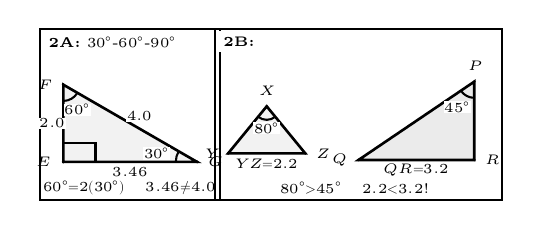
\begin{tikzpicture}[scale=0.49, every node/.style={font=\tiny, text=black}]
  % POE 2A: 30-60-90
  \begin{scope}[shift={(0,0)}]
    \draw[black, line width=0.8pt] (-0.60,-0.98) rectangle (4.05,3.45);
    \node[anchor=north west, inner sep=2pt, fill=white] at (-0.54,3.40) {\textbf{2A:} $30^\circ\text{-}60^\circ\text{-}90^\circ$};
    \coordinate (E) at (0,0);
    \coordinate (G) at (3.4641,0);
    \coordinate (F) at (0,2.0);
    \fill[gray!10] (E) -- (F) -- (G) -- cycle;
    \draw[black, line width=0.95pt] (E) -- (F) -- (G) -- cycle;
    \rightbox[0.24]{F}{E}{G}
    \draw[black, line width=0.75pt] ($(F)+(-90:0.42)$) arc (-90:-30:0.42);
    \draw[black, line width=0.75pt] ($(G)+(150:0.55)$) arc (150:180:0.55);
    \fill[black] (E) circle (1.2pt) node[left=1pt] {$E$};
    \fill[black] (F) circle (1.2pt) node[left=1pt] {$F$};
    \fill[black] (G) circle (1.2pt) node[right=0.5pt] {$G$};
    \node[fill=white, inner sep=0.3pt] at (-0.28,1.00) {$2.0$};
    \node[fill=white, inner sep=0.3pt] at (1.73,-0.25) {$3.46$};
    \node[fill=white, inner sep=0.3pt] at (1.98,1.18) {$4.0$};
    \node[fill=white, inner sep=0.3pt] at (0.36,1.35) {$60^\circ$};
    \node[fill=white, inner sep=0.3pt] at (2.42,0.22) {$30^\circ$};
    \node[fill=white, inner sep=0.4pt] at (1.72,-0.68) {$60^\circ{=}2(30^\circ)$ តែ $3.46{\neq}4.0$};
  \end{scope}
  % POE 2B: Two separate triangles
  \begin{scope}[shift={(4.35,0)}]
    \draw[black, line width=0.8pt] (-0.42,-0.98) rectangle (7.02,3.45);
    \node[anchor=north west, inner sep=2pt, fill=white] at (-0.36,3.40) {\textbf{2B:} ២ ត្រីកោណដាច់ពីគ្នា};
    % Tiny XYZ
    \coordinate (Y) at (-0.08,0.22);
    \coordinate (Z) at (1.92,0.22);
    \coordinate (X) at (0.92,1.44);
    \fill[gray!10] (X) -- (Y) -- (Z) -- cycle;
    \draw[black, line width=0.95pt] (X) -- (Y) -- (Z) -- cycle;
    \draw[black, line width=0.75pt] ($(X)+(-130:0.35)$) arc (-130:-50:0.35);
    \fill[black] (X) circle (1.1pt) node[above=0.5pt] {$X$};
    \fill[black] (Y) circle (1.1pt) node[left=0.5pt] {$Y$};
    \fill[black] (Z) circle (1.1pt) node[right=0.5pt] {$Z$};
    \node[fill=white, inner sep=0.3pt] at (0.92,0.88) {$80^\circ$};
    \node[fill=white, inner sep=0.3pt] at (0.92,-0.06) {$YZ{=}2.2$};
    % Larger PQR
    \coordinate (Q) at (3.30,0.05);
    \coordinate (R) at (6.30,0.05);
    \coordinate (P) at (6.30,2.08);
    \fill[gray!16] (P) -- (Q) -- (R) -- cycle;
    \draw[black, line width=0.95pt] (P) -- (Q) -- (R) -- cycle;
    \draw[black, line width=0.75pt] ($(P)+(-146:0.42)$) arc (-146:-90:0.42);
    \fill[black] (P) circle (1.1pt) node[above=0.5pt] {$P$};
    \fill[black] (Q) circle (1.1pt) node[left=0.5pt] {$Q$};
    \fill[black] (R) circle (1.1pt) node[right=0.5pt] {$R$};
    \node[fill=white, inner sep=0.3pt] at (5.86,1.42) {$45^\circ$};
    \node[fill=white, inner sep=0.3pt] at (4.80,-0.22) {$QR{=}3.2$};
    \node[fill=white, inner sep=0.4pt] at (3.20,-0.68) {$80^\circ{>}45^\circ$ តែ $2.2{<}3.2$!};
  \end{scope}
\end{tikzpicture}}

% ៦. E3 Explain: ឧទាហរណ៍ផ្ទាល់ (ទំ.១៥៨) + Trichotomy 3 ករណី
\newcommand{\figExplainINEQ}{%
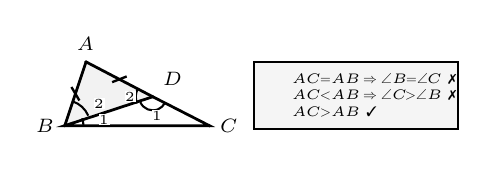
\begin{tikzpicture}[scale=0.54, every node/.style={font=\scriptsize, text=black}]
  % ឆ្វេង៖ រូបសម្រាយផ្ទាល់ (ទំ.១៥៨)
  \begin{scope}[shift={(-2.65,0)}]
    \coordinate (B) at (-1.35,0);
    \coordinate (C) at (2.05,0);
    \coordinate (A) at (-0.85,1.50);
    \coordinate (D) at (0.72,0.68);
    \fill[gray!10] (A) -- (B) -- (D) -- cycle;
    \draw[black, line width=1.0pt, tkslash] (A) -- (B);
    \draw[black, line width=1.0pt, tkslash] (A) -- (D);
    \draw[black, line width=1.0pt] (D) -- (C) -- (B) -- (D);
    \draw[black, line width=0.75pt] ($(B)+(0:0.44)$) arc (0:23:0.44);
    \draw[black, line width=0.75pt] ($(B)+(23:0.60)$) arc (23:72:0.60);
    \draw[black, line width=0.75pt] ($(D)+(152:0.40)$) arc (152:203:0.40);
    \draw[black, line width=0.75pt] ($(D)+(203:0.32)$) arc (203:332:0.32);
    \fill[black] (A) circle (1.2pt) node[above=0.5pt] {$A$};
    \fill[black] (B) circle (1.2pt) node[left=0.5pt] {$B$};
    \fill[black] (C) circle (1.2pt) node[right=0.5pt] {$C$};
    \fill[black] (D) circle (1.2pt) node[above right=0.5pt] {$D$};
    \node[font=\tiny, fill=white, inner sep=0.3pt] at (-0.54,0.52) {$2$};
    \node[font=\tiny, fill=white, inner sep=0.3pt] at (-0.42,0.14) {$1$};
    \node[font=\tiny, fill=white, inner sep=0.3pt] at (0.20,0.68) {$2$};
    \node[font=\tiny, fill=white, inner sep=0.3pt] at (0.82,0.24) {$1$};
  \end{scope}
  % ស្ដាំ៖ បីករណី Trichotomy (AC=AB? AC<AB? AC>AB!)
  \begin{scope}[shift={(1.80,0.08)}]
    \draw[black, line width=0.75pt, fill=gray!8] (-1.35,-0.15) rectangle (3.45,1.42);
    \node[font=\tiny, align=left] at (1.05,0.64) {%
      ករណី ១៖ $AC{=}AB \Rightarrow \ang{B}{=}\ang{C}$ \ding{55}\\
      ករណី ២៖ $AC{<}AB \Rightarrow \ang{C}{>}\ang{B}$ \ding{55}\\
      ករណី ៣៖ $AC{>}AB$ \ding{51}};
  \end{scope}
\end{tikzpicture}}

% ៧. E4 Elaborate: លំហាត់គំរូ (ទំ.១៥៨--១៥៩) រូប △ABC 58°, 75°, 47°
\newcommand{\figModelINEQ}{%
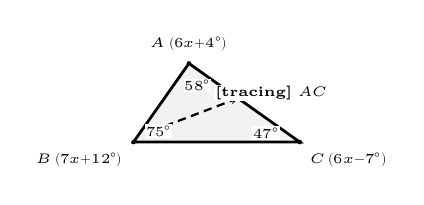
\begin{tikzpicture}[scale=0.64, every node/.style={font=\tiny, text=black}]
  \coordinate (B) at (-1.55,0);
  \coordinate (C) at (1.75,0);
  \coordinate (A) at (-0.45,1.56);
  \fill[gray!10] (A) -- (B) -- (C) -- cycle;
  \draw[black, line width=1.0pt] (A) -- (B) -- (C) -- cycle;
  \draw[black, line width=0.8pt, densely dashed, -{Stealth[length=3.2pt]}] (-1.18,0.22) -- (0.55,0.88);
  \fill[black] (A) circle (1.3pt) node[above=1pt] {$A\; (6x{+}4^\circ)$};
  \fill[black] (B) circle (1.3pt) node[below left=0.5pt] {$B\; (7x{+}12^\circ)$};
  \fill[black] (C) circle (1.3pt) node[below right=0.5pt] {$C\; (6x{-}7^\circ)$};
  \node[fill=white, inner sep=0.4pt] at (-0.28,1.12) {$58^\circ$};
  \node[fill=white, inner sep=0.4pt] at (-1.05,0.22) {$75^\circ$};
  \node[fill=white, inner sep=0.4pt] at (1.08,0.18) {$47^\circ$};
  \node[fill=white, inner sep=0.4pt] at (1.18,0.98) {\textbf{[tracing]} $AC$};
\end{tikzpicture}}

% ៨. E5 Evaluate: ប្រតិបត្តិ (ទំ.១៥៩) មុំទាល ∠BAC = 108° ពិតប្រាកដ (Erratum #3)
\newcommand{\figPracticeINEQ}{%
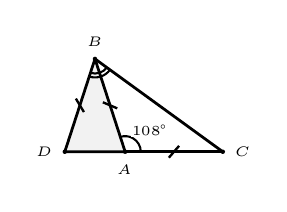
\begin{tikzpicture}[scale=0.62, every node/.style={font=\tiny, text=black}]
  \coordinate (A) at (0,0);
  \coordinate (C) at (2.00,0);
  \coordinate (B) at (-0.6180,1.9021);
  \coordinate (D) at (-1.2361,0);
  \fill[gray!10] (B) -- (D) -- (A) -- cycle;
  \draw[black, line width=1.0pt, tkslash] (B) -- (D);
  \draw[black, line width=1.0pt, tkslash] (A) -- (B);
  \draw[black, line width=1.0pt, tkslash] (A) -- (C);
  \draw[black, line width=1.0pt] (D) -- (A) (B) -- (C);
  \draw[black, line width=0.75pt] ($(A)+(0:0.32)$) arc (0:108:0.32);
  \draw[black, line width=0.75pt] ($(B)+(-108:0.30)$) arc (-108:-36:0.30);
  \draw[black, line width=0.75pt] ($(B)+(-108:0.38)$) arc (-108:-36:0.38);
  \fill[black] (A) circle (1.3pt) node[below=1pt] {$A$};
  \fill[black] (B) circle (1.3pt) node[above=1pt] {$B$};
  \fill[black] (C) circle (1.3pt) node[right=1pt] {$C$};
  \fill[black] (D) circle (1.3pt) node[left=1pt] {$D$};
  \node[fill=white, inner sep=0.4pt] at (0.50,0.44) {$108^\circ$};
\end{tikzpicture}}

% ៩. E5 Evaluate: កាតត្រួតពិនិត្យ A–D
\newcommand{\figExitCardsINEQ}{%
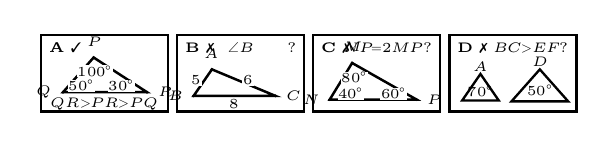
\begin{tikzpicture}[scale=0.58, every node/.style={font=\tiny, text=black}]
  % កាត A: PQR 100°, 50°, 30° => QR>PR>PQ ✓
  \begin{scope}[shift={(0,0)}]
    \draw[black, line width=0.85pt] (0,0) rectangle (2.78,1.68);
    \node[anchor=north west, inner sep=2pt] at (0.04,1.64) {\textbf{A} \ding{51}};
    \coordinate (P) at (1.15,1.18);
    \coordinate (Q) at (0.48,0.42);
    \coordinate (R) at (2.32,0.42);
    \draw[black, line width=0.9pt] (P) -- (Q) -- (R) -- cycle;
    \fill[black] (P) circle (1.0pt) node[above=0.5pt] {$P$};
    \fill[black] (Q) circle (1.0pt) node[left=0.5pt] {$Q$};
    \fill[black] (R) circle (1.0pt) node[right=0.5pt] {$R$};
    \node[fill=white, inner sep=0.3pt] at (1.18,0.88) {$100^\circ$};
    \node[fill=white, inner sep=0.3pt] at (0.88,0.56) {$50^\circ$};
    \node[fill=white, inner sep=0.3pt] at (1.76,0.56) {$30^\circ$};
    \node at (1.39,0.16) {$QR{>}PR{>}PQ$};
  \end{scope}
  % កាត B: Opposite-Vertex Trap AB=5, BC=8, AC=6 -> claims ∠B largest ✗
  \begin{scope}[shift={(2.98,0)}]
    \draw[black, line width=0.85pt] (0,0) rectangle (2.78,1.68);
    \node[anchor=north west, inner sep=2pt] at (0.04,1.64) {\textbf{B} \ding{55}};
    \coordinate (A) at (0.76,0.92);
    \coordinate (B) at (0.36,0.34);
    \coordinate (C) at (2.15,0.34);
    \draw[black, line width=0.9pt] (A) -- (B) -- (C) -- cycle;
    \fill[black] (A) circle (1.0pt) node[above=0.5pt] {$A$};
    \fill[black] (B) circle (1.0pt) node[left=0.5pt] {$B$};
    \fill[black] (C) circle (1.0pt) node[right=0.5pt] {$C$};
    \node[fill=white, inner sep=0.3pt] at (0.42,0.68) {$5$};
    \node[fill=white, inner sep=0.3pt] at (1.55,0.68) {$6$};
    \node[fill=white, inner sep=0.3pt] at (1.25,0.16) {$8$};
    \node[anchor=north east, inner sep=2pt] at (2.74,1.64) {$\ang{B}$ ធំបំផុត?};
  \end{scope}
  % កាត C: False Ratio Trap MNP 80°, 40°, 60° -> NP=2MP? ✗
  \begin{scope}[shift={(5.96,0)}]
    \draw[black, line width=0.85pt] (0,0) rectangle (2.78,1.68);
    \node[anchor=north west, inner sep=2pt] at (0.04,1.64) {\textbf{C} \ding{55}};
    \coordinate (M) at (0.85,1.06);
    \coordinate (N) at (0.36,0.26);
    \coordinate (P) at (2.26,0.26);
    \draw[black, line width=0.9pt] (M) -- (N) -- (P) -- cycle;
    \fill[black] (M) circle (1.0pt) node[above=0.5pt] {$M$};
    \fill[black] (N) circle (1.0pt) node[left=0.5pt] {$N$};
    \fill[black] (P) circle (1.0pt) node[right=0.5pt] {$P$};
    \node[fill=white, inner sep=0.2pt] at (0.90,0.74) {$80^\circ$};
    \node[fill=white, inner sep=0.2pt] at (0.82,0.39) {$40^\circ$};
    \node[fill=white, inner sep=0.2pt] at (1.76,0.39) {$60^\circ$};
    \node[anchor=north east, inner sep=2pt] at (2.74,1.64) {$NP{=}2MP?$};
  \end{scope}
  % កាត D: Two-Triangles Trap ABC (∠A=70°) vs large DEF (∠D=50°) ✗
  \begin{scope}[shift={(8.94,0)}]
    \draw[black, line width=0.85pt] (0,0) rectangle (2.78,1.68);
    \node[anchor=north west, inner sep=2pt] at (0.04,1.64) {\textbf{D} \ding{55}};
    \coordinate (A) at (0.68,0.82);
    \coordinate (B) at (0.28,0.24);
    \coordinate (C) at (1.08,0.24);
    \draw[black, line width=0.85pt] (A) -- (B) -- (C) -- cycle;
    \node at (0.68,0.98) {$A$};
    \node at (0.68,0.44) {$70^\circ$};
    \coordinate (D) at (1.98,0.92);
    \coordinate (E) at (1.36,0.22);
    \coordinate (F) at (2.60,0.22);
    \draw[black, line width=0.85pt] (D) -- (E) -- (F) -- cycle;
    \node at (1.98,1.08) {$D$};
    \node at (1.98,0.46) {$50^\circ$};
    \node[anchor=north east, inner sep=2pt] at (2.74,1.64) {$BC{>}EF?$};
  \end{scope}
\end{tikzpicture}}

% ១០. ជំហានទី៥ កិច្ចការផ្ទះ៖ លំហាត់ទី១៣, ទី១៤ និងទី១៥ (ទំ.១៦៦)
\newcommand{\figHWnewINEQ}{%
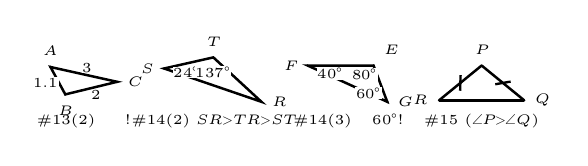
\begin{tikzpicture}[scale=0.47, every node/.style={font=\tiny, text=black}]
  % ទី១៣ (២) ABC 1.1m, 2m, 3m
  \begin{scope}[shift={(-5.45,0)}]
    \coordinate (A) at (-0.65,0.92);
    \coordinate (B) at (-0.25,0.18);
    \coordinate (C) at (1.15,0.52);
    \draw[black, line width=0.9pt] (A) -- (B) -- (C) -- cycle;
    \fill[black] (A) circle (1.0pt) node[above=0.5pt] {$A$};
    \fill[black] (B) circle (1.0pt) node[below=0.5pt] {$B$};
    \fill[black] (C) circle (1.0pt) node[right=0.5pt] {$C$};
    \node[fill=white, inner sep=0.3pt] at (-0.78,0.50) {$1.1$};
    \node[fill=white, inner sep=0.3pt] at (0.58,0.16) {$2$};
    \node[fill=white, inner sep=0.3pt] at (0.35,0.90) {$3$};
    \node at (0.25,-0.55) {\#13(2) មើលលេខ!};
  \end{scope}
  % ទី១៤ (២) STR 24°, 137°, 19°
  \begin{scope}[shift={(-1.75,0)}]
    \coordinate (S) at (-1.28,0.88);
    \coordinate (T) at (0.05,1.18);
    \coordinate (R) at (1.35,-0.02);
    \draw[black, line width=0.9pt] (S) -- (T) -- (R) -- cycle;
    \fill[black] (S) circle (1.0pt) node[left=0.5pt] {$S$};
    \fill[black] (T) circle (1.0pt) node[above=0.5pt] {$T$};
    \fill[black] (R) circle (1.0pt) node[right=0.5pt] {$R$};
    \node[fill=white, inner sep=0.2pt] at (-0.68,0.77) {$24^\circ$};
    \node[fill=white, inner sep=0.2pt] at (0.05,0.78) {$137^\circ$};
    \node at (0.05,-0.55) {\#14(2) $SR{>}TR{>}ST$};
  \end{scope}
  % ទី១៤ (៣) FEG 40°, 80°, 60° (កែ 50°->60°)
  \begin{scope}[shift={(1.95,0)}]
    \coordinate (F) at (-1.10,0.96);
    \coordinate (E) at (0.68,0.96);
    \coordinate (G) at (1.05,-0.02);
    \draw[black, line width=0.9pt] (F) -- (E) -- (G) -- cycle;
    \fill[black] (F) circle (1.0pt) node[left=0.5pt] {$F$};
    \fill[black] (E) circle (1.0pt) node[above right=0.5pt] {$E$};
    \fill[black] (G) circle (1.0pt) node[right=0.5pt] {$G$};
    \node[fill=white, inner sep=0.3pt] at (-0.48,0.75) {$40^\circ$};
    \node[fill=white, inner sep=0.3pt] at (0.44,0.72) {$80^\circ$};
    \node[fill=white, inner sep=0.3pt] at (0.55,0.22) {$60^\circ$};
    \node at (0.00,-0.55) {\#14(3) កែ $60^\circ$!};
  \end{scope}
  % ទី១៥ PQR: QR>QP, PR=PQ
  \begin{scope}[shift={(5.55,0)}]
    \coordinate (P) at (0,0.96);
    \coordinate (R) at (-1.15,0.02);
    \coordinate (Q) at (1.15,0.02);
    \draw[black, line width=0.9pt, tkslash] (P) -- (R);
    \draw[black, line width=0.9pt, tkslash] (P) -- (Q);
    \draw[black, line width=0.9pt] (R) -- (Q);
    \fill[black] (P) circle (1.0pt) node[above=0.5pt] {$P$};
    \fill[black] (R) circle (1.0pt) node[left=0.5pt] {$R$};
    \fill[black] (Q) circle (1.0pt) node[right=0.5pt] {$Q$};
    \node at (0,-0.55) {\#15 ($\ang{P}{>}\ang{Q}$)};
  \end{scope}
\end{tikzpicture}}

% ============================================================================
% ចាប់ផ្ដើមឯកសារ (Document Body)
% ============================================================================
\begin{document}
\fontsize{9.5pt}{14.0pt}\selectfont

% -------------------- ក្បាលកិច្ចតែងការ (Header) --------------------
\begin{center}
  {\muol\fontsize{11pt}{16pt}\selectfont ព្រះរាជាណាចក្រកម្ពុជា}\\[2pt]
  {\muol\fontsize{10pt}{15pt}\selectfont ជាតិ សាសនា ព្រះមហាក្សត្រ}\\[1pt]
  \khmflourish
\end{center}

\vspace{-15pt}
{\muol\fontsize{9.5pt}{13.2pt}\selectfont
មន្ទីរអប់រំ យុវជន និងកីឡា ខេត្តកំពង់ធំ\\
ការិយាល័យអប់រំ យុវជន និងកីឡា ស្រុកកំពង់ស្វាយ\\
អនុវិទ្យាល័យព្រះក្រសាំង}

\vspace{2pt}
\begin{center}
  {\muol\fontsize{10pt}{15pt}\selectfont កិច្ចតែងការបង្រៀន}
\end{center}
\vspace{1pt}

% -------------------- ព័ត៌មានទូទៅ (Metadata) --------------------
{\renewcommand{\arraystretch}{1.04}
\hspace*{4.05cm}%
\begin{tabular}{@{}l l l@{}}
  - \hspace{0.35cm} មុខវិជ្ជា & : & គណិតវិទ្យា ថ្នាក់ទី៨ \\
  - \hspace{0.35cm} ចំណងជើងមេរៀន & : & មេរៀនទី១២ ការប្រៀបធៀបត្រីកោណ \\
  - \hspace{0.35cm} ចំណងជើងរង & : & ៣. វិសមភាពក្នុងត្រីកោណ \\
  & & ៣.១ វិសមភាពចំពោះជ្រុងនិងមុំនៃត្រីកោណមួយ \\
  - \hspace{0.35cm} រយៈពេល & : & ១ ម៉ោងសិក្សា (៥០ នាទី) \\
  - \hspace{0.35cm} បង្រៀនដោយ & : & ហុក ប៊ុនថែន \\
  - \hspace{0.35cm} កាលបរិច្ឆេទ & : & ថ្ងៃព្រហស្បតិ៍ ទី៣ ខែធ្នូ ឆ្នាំ២០២៦ \\
\end{tabular}

\vspace{2pt}

% -------------------- I. វត្ថុបំណង --------------------
\textbf{I.} {\muol វត្ថុបំណង}\\[1.5pt]
\hspace*{0.55cm}%
\begin{tabular}{@{}l l L{14.2cm}@{}}
  \wcirc \hspace{0.25cm} វិជ្ជាសម្បទា & : & សិស្សប្រាប់និងស្រាយទ្រឹស្ដីបទផ្ទាល់ ($AC>AB\Rightarrow\ang{B}>\ang{C}$ តាម $AD=AB<AC$ និងមុំក្រៅ) និងច្រាស ($\ang{B}>\ang{C}\Rightarrow AC>AB$ តាម ៣ ករណី កែពាក្យ «ក៏មិនប៉ុនគ្នាដែរ») ក្នុងត្រីកោណតែមួយ ។ \\
  \wcirc \hspace{0.25cm} បំណិនសម្បទា & : & សិស្សបត់ $1:1$ ($\tri{ABC}$), ធ្វើ POE ($30^\circ\text{-}60^\circ\text{-}90^\circ$ vs ២ ត្រីកោណ), ប្រើ \textbf{[tracing]}, តារាងអក្សរឈម និង \cnum{1}--\cnum{5} ដោះស្រាយគំរូ ($x=9^\circ\Rightarrow AC>BC>AB$), ប្រតិបត្តិ ($108^\circ, BD<BC$) និង \#13--\#15 ។ \\
  \wcirc \hspace{0.25cm} ចរិយាសម្បទា & : & សហការជា «ក្រុមអ្នកបច្ចេកទេសដងស្ទូច និងទ្វារបត់មុំ» តាមវិន័យ \en{Pause-Ask / Pause-Review} ដោយជឿតម្លៃលេខជាងរូបគំនូរ និងចៀសវាងអន្ទាក់គុណសមាមាត្រ ។ \\
\end{tabular}

\vspace{1.5pt}

% -------------------- II. សម្ភារៈឧបទេស --------------------
\textbf{II.} {\muol សម្ភារៈឧបទេស}\\[1.5pt]
\hspace*{0.55cm}$\bullet$ \hspace{0.35cm} សៀវភៅគោលទី៨ (ទំ.១៥៨--១៥៩, ១៦៤--១៦៦) បន្ទាត់ក្រិត ១:១ រ៉ាព័រទ័រ កន្ត្រៃ កញ្ចប់ ១:១ (ទំព័រ ១) កាត E4 (ទំព័រ ២) សន្លឹក E5 (ទំព័រ ៣) ផ្ទាំង \cnum{1}--\cnum{5} (ទំព័រ ៤) កាត A--D (ទំព័រ ៥) និងប័ណ្ណកិច្ចការផ្ទះ (ទំព័រ ៦)

\vspace{1.5pt}

% -------------------- III. វិធីសាស្រ្តបង្រៀន --------------------
\textbf{III.} {\muol វិធីសាស្រ្តបង្រៀន}\\[1.5pt]
\hspace*{0.55cm}%
\begin{tabular}{@{}l l l@{}}
  $\bullet$ \hspace{0.35cm} គោលវិធី & : \hspace{0.7cm} & សិស្សមជ្ឈមណ្ឌល \\
  $\bullet$ \hspace{0.35cm} យុទ្ធវិធីបង្រៀន & : & ស្ថាបនានិយម គម្រូ 5Es (បត់/រំកិល ១:១ $AD=AB$, Dual POE, \textbf{[tracing]}, តារាងអក្សរឈម និង ៣ តួនាទី) \\
\end{tabular}
}

\vspace{1.5pt}

% -------------------- IV. ដំណើរការបង្រៀន --------------------
\textbf{IV.} {\muol ដំណើរការបង្រៀន}

\vspace{-3pt}

% ============================================================================
% តារាងដំណើរការបង្រៀន (Modular Multi-Row 3-Column Table – 50 នាទី)
% ============================================================================
\renewcommand{\arraystretch}{1.04}
\begin{longtable}{|L{5.50cm}|L{7.90cm}|L{4.80cm}|}
\hline
\rowcolor{headgray}
\multicolumn{1}{|c|}{\muol សកម្មភាពគ្រូ} &
\multicolumn{1}{c|}{\muol ខ្លឹមសារមេរៀន} &
\multicolumn{1}{c|}{\muol សកម្មភាពសិស្ស} \\
\hline
\endfirsthead

\hline
\endhead

\hline
\endfoot

\hline
\endlastfoot

% ==================== ជំហានទី១ (2min) ====================
\stepheader{ជំហានទី១ \enbf{(}រដ្ឋបាលថ្នាក់\enbf{)}}
- ពិនិត្យអវត្តមាន សណ្ដាប់ធ្នាប់ និងសុវត្ថិភាពកន្ត្រៃ \newline
- ចាត់ក្រុម ៣ នាក់ («ក្រុមអ្នកបច្ចេកទេសដងស្ទូច និងទ្វារបត់មុំ») និងចែកកញ្ចប់ ១:១ (ទំព័រ ១) ដាក់ផ្កាប់លើតុ
&
\hspace*{0.3cm}- រដ្ឋបាលថ្នាក់ \newline
\hspace*{0.3cm}- អនាម័យ និងសុវត្ថិភាពកន្ត្រៃ \newline
\hspace*{0.3cm}- ត្រៀមក្រុមអ្នកបច្ចេកទេសដងស្ទូច និងទ្វារបត់មុំ
&
- រាយការណ៍អវត្តមាន \newline
- អង្គុយតាមក្រុម ៣ នាក់ \\
\hline

% ==================== ជំហានទី២ (9min: <=3 + 3 + E1 3) ====================
\stepheader{ជំហានទី២ \enbf{(}កិច្ចការផ្ទះ \enbf{+} ទំនាក់ទំនងមេរៀនថ្មី\enbf{)}}
% --- ២.១ កំណែកិច្ចការផ្ទះមេរៀនមុន (<=3min) ---
\ditem \textbf{កំណែកិច្ចការផ្ទះ ($\le 3\unit{min}$)} ៖ \newline
+ ផ្ទៀង \textbf{លំហាត់ទី២} (ទំ.១៦៤) និង \textbf{ទី៨, ទី១១} (ទំ.១៦៥) \newline
+ \textbf{សំណួរបញ្ឆោត (ទី២)}៖ «ហេតុអ្វីក្នុងលំហាត់ទី២ មិនអាចប្រើ \textbf{ជ.ជ.ម} ផ្ទាល់លើ $\ang{PSQ}=\ang{PTR}$ បាន?» \newline
\timenote{កុំឱ្យសរសេរវែងលើក្ដារខៀន}
&
\centerline{\redsub{កំណែកិច្ចការផ្ទះមេរៀនមុន (ទំ.១៦៤--១៦៥)}}
\cfig{\figHWoldINEQ}
{\footnotesize - \textbf{ទី២}៖ $PQ=PR, PS=PT$ ផ្គុំមុំចន្លោះ $\ang{P}$ រីឯ $\ang{PSQ}=\ang{PTR}$ ជាមុំក្រៅចន្លោះ (\textit{អន្ទាក់ \en{SSA}})! ត្រូវរក $\ang{Q}=\ang{R}$ និងតាម $180^\circ$ បាន $\ang{QPS}=\ang{RPT} \Rightarrow \tri{PQS}\cg\tri{PRT}$ (\textbf{ជ.ម.ជ / ម.ជ.ម}) ។ \newline
- \textbf{ទី៨}៖ $\tri{MBC}\cg\tri{NCB}$ (\textbf{ជ.ម.ជ}) $\Rightarrow \tri{PBC}$ សមបាទ ។ \textbf{ទី១១}៖ $\tri{HOE}\cg\tri{DBP}$ (\textbf{ជ.ម.ជ}) $\Rightarrow \tri{FPE}$ សមបាទ ។}
&
- ផ្ទៀង និងឆ្លើយ៖ «ជ្រុង $PQ, PS$ ផ្គុំមុំ $\ang{P}$ — មិនមែន $\ang{PSQ}$ ទេ ត្រូវភ្ជាប់គូមុំត្រឹមត្រូវ!» \\[-2pt]

% --- ២.២ រំលឹកមេរៀនទាក់ទង (3min) ---
\ditem \textbf{រំលឹករហ័ស (3min)} ៖ \newline
+ មុំក្រៅត្រីកោណ ($\ang{D_2}=\ang{B_1}+\ang{C}$) \newline
+ មុំបាទសមបាទ ($AD=AB$) \newline
+ \textbf{ក្បួនអក្សរទី៣ ដែលបាត់} ក្នុង $\tri{ABC}$ \newline
\timenote{សរុបកុំឱ្យលើស 3min}
&
\centerline{\redsub{រំលឹកមេរៀនទាក់ទងមេរៀនថ្មី}}
\cfig{\figPrereqINEQ}
{\footnotesize - \textbf{មុំក្រៅ}៖ $\ang{D_2}=\ang{B_1}+\ang{C} \Rightarrow \ang{D_2}>\ang{C}$ \quad \textbar{} \quad \textbf{សមបាទ}៖ $AD=AB \Rightarrow \ang{B_2}=\ang{D_2}$ \newline
- \textbf{ក្បួនអក្សរទី៣ ដែលបាត់}៖ ក្នុង $\tri{ABC}$, $\ang{A}\leftrightarrow BC$ (បាត់ $B,C$), $\ang{B}\leftrightarrow AC$ (បាត់ $A,C$), $\ang{C}\leftrightarrow AB$ (បាត់ $A,B$)}
&
- ឆ្លើយ៖ «$\ang{D_2}>\ang{C}$; $\ang{B_2}=\ang{D_2}$; មុំឈមជ្រុងគឺប្រើអក្សរទី៣ ដែលបាត់!» \\[-2pt]

% --- ២.៣ E1 Engage: ដងស្ទូច និងខ្សែរ៉កបើកមុំទ្វារទឹក ---
\fiveE{E1 - Engage (3min)} \newline
\ditem \textbf{ដងស្ទូច និងខ្សែរ៉កបើកមុំទ្វារទឹក (កំពង់ស្វាយ)} ៖ \newline
បង្ហាញដងស្ទូចដៃជាប់ $4\unit{m}$ និង $7\unit{m}$ លើ ២ ទីតាំង ($30^\circ$ vs $60^\circ$) ហើយសួរទាយ ៖ \newline
(១) ក្នុងត្រីកោណតែមួយ ហេតុអ្វីមុំបើកធំជាង តែងតែទាញខ្សែរ៉កឈមវែងជាង? \newline
(២) បើមុំកើនគុណ ២ ($30^\circ \to 60^\circ$) តើខ្សែរ៉កវែងគុណ ២ ដែរឬទេ? \timenote{(កុំទាន់ផ្ដល់ចម្លើយ)}
&
\centerline{\redsub{ស្ថានភាពពិត៖ ដងស្ទូច និងខ្សែរ៉កបើកមុំទ្វារទឹក}}
\cfig{\figEngageINEQ}
\hspace*{0.1cm}\textbf{ចម្ងល់} ៖ (១) ក្នុង $\tri{ABC}$ ($AC=7\unit{m}>AB=4\unit{m}$) ហេតុអ្វី $\ang{B}>\ang{C}$? (២) មុំ $30^\circ \to 60^\circ$ តើ $B'C'=2BC$ មែនទេ?
&
- ស្រង់ការទស្សន៍ទាយរបស់ក្រុម ទាំងសំណួរ (១) និង (២) \\
\hline

% ==================== ជំហានទី៣ (17min: E2 11m + E3 6m) ====================
\stepheader{ជំហានទី៣ \enbf{(}ខ្លឹមសារមេរៀនថ្មី\enbf{)}}
% --- ៣.១ ចំណងជើង & E2 Act 1 (6min) ---
- សរសេរចំណងជើងមេរៀនលើក្ដារខៀន \newline
\fiveE{E2 - Explore (11min)} \newline
\ditem \textbf{សកម្មភាព ១៖ កាត់បត់ ១:១ (6min)} \newline
+ ផ្ទៀងក្រិត $5.00\unit{cm}$ (\en{Actual Size 100\%}, ទំព័រ ១) \newline
+ កាត់ $\tri{ABC}$ ($AB=4.00, BC=5.50, AC=6.50\unit{cm}$) រំកិល/បត់ $AB$ លើ $AC$ គូសចំណុចជំនួយ $D$ ($AD=AB=4.00\unit{cm}<AC$) និងផ្នត់ $BD$
&
មេរៀនទី១២ \hspace{0.1cm} {\muol ការប្រៀបធៀបត្រីកោណ} \textbf{(ត)} \newline
៣. វិសមភាពក្នុងត្រីកោណ \newline
៣.១ វិសមភាពចំពោះជ្រុងនិងមុំនៃត្រីកោណមួយ \par\vspace*{1pt}
\cfig{\figExploreOneINEQ}
{\footnotesize \hspace*{0.1cm}+ ព្រោះ $AD=AB=4.00\unit{cm} < AC=6.50\unit{cm}$, ចំណុច $D$ ស្ថិតនៅ\textbf{ចន្លោះ} $A$ និង $C$ ។ \newline
\hspace*{0.1cm}+ \graybox{$\tri{ABD}$ សមបាទ} $\Rightarrow \ang{B_2}=\ang{D_2}$; មុំក្រៅ $\tri{BCD}$ $\Rightarrow \ang{D_2}=\ang{B_1}+\ang{C}>\ang{C}$; បូកមុំ $\ang{B}=\ang{B_1}+\ang{B_2}>\ang{B_2}>\ang{C}$ ។}
&
- កត់ចំណងជើង \newline
- បត់ $AB$ លើ $AC$ គូស $D, BD$ និងផ្ទៀង $\ang{B}>\ang{B_2}=\ang{D_2}>\ang{C}$ \\[-2pt]

% --- ៣.២ E2 Act 2 Dual POE (5min) ---
\ditem \textbf{សកម្មភាព ២៖ Dual POE (5min)} \newline
+ \textbf{POE 2A (អន្ទាក់គុណសមាមាត្រ)}៖ ទាយហើយវាស់ $\tri{EFG}$ $30^\circ\text{-}60^\circ\text{-}90^\circ$ ($1:1$) ៖ តើ $EG=2EF$ និង $FG=3EF$ ទេ? \newline
+ \textbf{POE 2B (អន្ទាក់ ២ ត្រីកោណ)}៖ ធៀប $\tri{XYZ}$ តូច ($\ang{X}=80^\circ$) នឹង $\tri{PQR}$ ធំ ($\ang{P}=45^\circ$) ៖ តើ $YZ>QR$ ទេ?
&
{\centering\textbf{POE 2A (មុំគុណ $\neq$ ជ្រុងគុណ) vs POE 2B (២ ត្រីកោណដាច់ពីគ្នា)}\par}
\cfig{\figExploreTwoINEQ}
{\footnotesize - \textbf{POE 2A}៖ $\ang{F}=60^\circ=2\ang{G}$ តែ $EG\approx 3.46 \neq 2(2.00)$; $\ang{E}=90^\circ=3\ang{G}$ តែ $FG=4.00 \neq 3(2.00)$ $\Rightarrow$ \graybox{លំដាប់ត្រូវ តែសមាមាត្រខុស!} \newline
- \textbf{POE 2B}៖ $\ang{X}=80^\circ>\ang{P}=45^\circ$ តែ $YZ=2.20<QR=3.20$ $\Rightarrow$ ទ្រឹស្ដីប្រើបាន\textbf{តែក្នុងត្រីកោណតែមួយ}!}
&
- ទាយ-វាស់-ពន្យល់៖ បដិសេធសមាមាត្រលីនេអ៊ែរ និងការប្រៀបធៀបឆ្លងត្រីកោណ \\[-2pt]

% --- ៣.៣ E3 Explain: ឧទាហរណ៍សម្រាយផ្ទាល់ + ប្រអប់ទ្រឹស្ដីបទ (Erratum #1) ---
\fiveE{E3 - Explain (6min)} \newline
\ditem \textbf{បង្គុំសម្រាយផ្ទាល់ (ឧទាហរណ៍ ទំ.១៥៨)} \newline
+ ប្រើ \textbf{[tracing]} លើ $\ang{B}=\ang{B_1}+\ang{B_2}$ \newline
+ បញ្ជាក់ហេតុផលចំណុចចន្លោះ $AD=AB<AC$ \newline
\ditem \textbf{ប្រអប់ទ្រឹស្ដីបទ ៣.១ និងសម្រាយច្រាស ៣ ករណី} \newline
\timenote{(កែខុសទំ.១៥៨៖ «ក៏មានប៉ុនគ្នាដែរ» $\to$ «ក៏មិនប៉ុនគ្នាដែរ» និងបំពេញ «។»)}
&
\textbf{ឧទាហរណ៍ (ទំ.១៥៨)៖} ក្នុង $\tri{ABC}$ ដែល $AC>AB$ ($\ang{B}$ ឈម $AC$, $\ang{C}$ ឈម $AB$) ។ បង្ហាញថា $\ang{B}>\ang{C}$ ។
\cfig{\figExplainINEQ}
{\footnotesize - ដៅ $D\in AC$ ដែល $AD=AB$ (ដោយ $AD=AB<AC$ នោះ $D$ ចន្លោះ $A,C$) $\Rightarrow \tri{ABD}$ សមបាទកំពូល $A \Rightarrow \ang{B_2}=\ang{D_2}$ ។ \newline
- ដោយ $\ang{D_2}$ ជាមុំក្រៅ $\tri{BCD} \Rightarrow \ang{D_2}=\ang{B_1}+\ang{C}>\ang{C} \Rightarrow \ang{B_2}>\ang{C}$ (១) ។ \newline
- តាម \textbf{[tracing]} $\ang{B}=\ang{B_1}+\ang{B_2}>\ang{B_2}$ (២) ។ ពី (១),(២) បាន \graybox{$\ang{B}>\ang{C}$} ។ \newline
\textbf{ទ្រឹស្ដីបទ (ទំ.១៥៨ កែតម្រូវ)៖} ក្នុងត្រីកោណមួយ \newline
$\bullet$ បើជ្រុងពីរមិនប៉ុនគ្នា មុំដែលឈមនឹងជ្រុងទាំងពីរនេះក៏មិនប៉ុនគ្នាដែរ ហើយមុំដែលឈមនឹងជ្រុងធំជាង ជាមុំធំជាង \textbf{។} \newline
$\bullet$ ច្រាសមកវិញ បើមុំពីរមិនប៉ុនគ្នា ជ្រុងដែលឈមនឹងមុំទាំងពីរនេះ\graybox{\textbf{ក៏មិនប៉ុនគ្នាដែរ}} ហើយជ្រុងដែលឈមនឹងមុំធំជាង ជាជ្រុងធំជាង ។ \newline
\textbf{សម្រាយច្រាស ($\ang{B}>\ang{C}\Rightarrow AC>AB$)៖} បដិសេធករណី ១ ($AC=AB\Rightarrow\ang{B}=\ang{C}$) និងករណី ២ ($AC<AB\Rightarrow\ang{C}>\ang{B}$) នាំឱ្យសល់ករណី ៣ ($AC>AB$) ។}
&
- គូស \textbf{[tracing]} កត់សម្រាយផ្ទាល់ និងកែពាក្យខុសក្នុងសៀវភៅទំ.១៥៨ រួចកត់ ៣ ករណី \\[-2pt]

% --- ៣.៤ E3 Explain: ក្បួនអក្សរទី៣បាត់ & ធនាគារហេតុផល ①–⑤ ---
\cnum{1} បញ្ជាក់ \textbf{ក្បួនអក្សរទី៣ ដែលបាត់} \newline
\cnum{2} បិទផ្ទាំង \textbf{ធនាគារហេតុផល \cnum{1}--\cnum{5}} (ទំព័រ ៤)
&
{\footnotesize\textbf{ធនាគារហេតុផល \cnum{1}--\cnum{5}៖} \cnum{1} ស្ពានមុំឈម–ជ្រុងឈម (ក្បួនអក្សរទី៣ ដែលបាត់ក្នុងត្រីកោណតែមួយ) $\vert$ \cnum{2} ទ្រឹស្ដីបទផ្ទាល់ ៣.១ (ក្នុងត្រីកោណមួយ ជ្រុងធំជាង $\Rightarrow$ មុំឈមធំជាង) $\vert$ \cnum{3} ទ្រឹស្ដីបទច្រាស ៣.១ (ក្នុងត្រីកោណមួយ មុំធំជាង $\Rightarrow$ ជ្រុងឈមធំជាង — ក៏មិនប៉ុនគ្នាដែរ) $\vert$ \cnum{4} សំណង់ចំណុចជំនួយ និងមុំក្រៅត្រីកោណ ($AD=AB<AC$, $\ang{}$ក្រៅ $>\ang{}$ក្នុងមិនជាប់) $\vert$ \cnum{5} ផលបូកមុំក្នុងត្រីកោណ $180^\circ$ / បីករណី (\en{Trichotomy}) / ស្ពានជំនួសអង្កត់ស្មើគ្នា ។}
&
- ផ្ទៀង \cnum{1}--\cnum{5} លើផ្ទាំងទំព័រ ៤ \\
\hline

% ==================== ជំហានទី៤ (20min: E4 10m + E5 10m) ====================
\stepheader{ជំហានទី៤ \enbf{(}ពង្រីកចំណេះដឹង\enbf{)}}
% --- ៤.១ E4 Elaborate: លំហាត់គំរូ (ទំ.១៥៨--១៥៩, Erratum #2) ---
\fiveE{E4 - Elaborate (10min)} \newline
\ditem ចែកកាត \textbf{«លំហាត់គំរូ»} (ទំព័រ ២) ៖ \newline
\hspace*{0.1cm}\cnum{1} គណនា $x$ តាមផលបូកមុំ $180^\circ$ \timenote{(បំពេញ $9^\circ$ កុំភ្លេច $^\circ$ ដូចទំ.១៥៩!)} \newline
\hspace*{0.1cm}\cnum{2} បំពេញ \textbf{តារាងអក្សរឈម ៣ ជួរ} និង \textbf{[tracing]} \newline
\hspace*{0.1cm}\cnum{3} សួរ \textbf{EIA 30s} ការពារកំហុសអក្សរឈម និងសមាមាត្រ
&
{\muol លំហាត់គំរូ} \textbf{(ទំ.១៥៨--១៥៩ កែតម្រូវ) ៖} ក្នុង $\tri{ABC}$ មាន $\ang{A}=6x+4^\circ, \ang{B}=7x+12^\circ, \ang{C}=6x-7^\circ$ ។ ចូររៀបជ្រុងនៃ $\tri{ABC}$ តាមលំដាប់ពីធំទៅតូច ។
\cfig{\figModelINEQ}
{\footnotesize + $\ang{A}+\ang{B}+\ang{C}=180^\circ \Rightarrow 19x+9^\circ=180^\circ \Rightarrow 19x=180^\circ-$\graybox{$9^\circ$}$ =171^\circ \Rightarrow x=9^\circ$ (\cnum{5}) ។ \newline
+ នោះ $\ang{A}=58^\circ, \ang{B}=75^\circ, \ang{C}=47^\circ$ ($58^\circ+75^\circ+47^\circ=180^\circ$) ។ \newline
{\scriptsize\setlength{\tabcolsep}{3.5pt}\renewcommand{\arraystretch}{1.05}%
\centering
\begin{tabular}{|c|c|c|}
  \hline
  \cellcolor{headgray}\textbf{មុំ ($\ang{B}>\ang{A}>\ang{C}$)} & \cellcolor{headgray}\textbf{កំពូលទី៣បាត់} & \cellcolor{headgray}\textbf{ជ្រុងឈម (\cnum{1}, \cnum{3})} \\
  \hline
  $\ang{B}=75^\circ$ (ធំបំផុត) & បាត់ $B \to A,C$ & $AC$ (វែងបំផុត) \\
  $\ang{A}=58^\circ$ (កណ្ដាល) & បាត់ $A \to B,C$ & $BC$ (កណ្ដាល) \\
  $\ang{C}=47^\circ$ (តូចបំផុត) & បាត់ $C \to A,B$ & $AB$ (ខ្លីបំផុត) \\[2pt]
  \hline
\end{tabular}}\par\vspace{1pt}
+ លំដាប់ពីធំទៅតូច៖ \graybox{$AC > BC > AB$} (\cnum{3}) ។ \newline
\timenote{EIA 30s៖ ហេតុអ្វី $\ang{B}$ ឈម $AC$ មិនមែន $AB$? ហើយតើ $AC/AB = 75^\circ/47^\circ$ ឬទេ?}}
&
- ដោះស្រាយ $x=9^\circ$, បំពេញតារាងអក្សរឈម ៣ ជួរ + \textbf{[tracing]} និងឆ្លើយ EIA 30s \\[-2pt]

% --- ៤.២ E5 Evaluate: ប្រតិបត្តិ (6.5min, ទំព័រ ៣) ---
\fiveE{E5 - Evaluate (10min)} \newline
\ditem {\muol លំហាត់ប្រតិបត្តិ} \textbf{(6.5min, ទំព័រ ៣)} \newline
ចែកសន្លឹក \textbf{«តុផ្ទៀងផ្ទាត់អក្សរឈម និងស្ពានអង្កត់ស្មើ ៣ តួនាទី»} (\en{Pause-Ask / Pause-Review})៖ \newline
\hspace*{0.05cm}\cnum{1} \textbf{តួនាទី ១ (\en{Pause-Ask})}៖ គូសដាន \textbf{[tracing]} $\tri{ABC}$ និង \cnum{1} \newline
\hspace*{0.05cm}\cnum{2} \textbf{តួនាទី ២}៖ ផ្គូផ្គងស្ពាន $AB=AC=BD$ \newline
\hspace*{0.05cm}\cnum{3} \textbf{តួនាទី ៣ (\en{Pause-Review})}៖ សរសេរសម្រាយ \cnum{3}, \cnum{5} និង \textbf{បិទ E1}
&
{\muol លំហាត់ប្រតិបត្តិ} \textbf{(ទំ.១៥៩ កែរូប $\ang{BAC}=108^\circ$)}៖ គេឱ្យ $D\text{-}A\text{-}C$ ត្រង់ជួរ, $AB=AC=BD$ និង $\ang{ABC}<\ang{BAC}$ ។ បង្ហាញថា $BD<BC$ ។
\cfig{\figPracticeINEQ}
{\footnotesize + ក្នុង $\tri{ABC}$, មាន $\ang{ABC}<\ang{BAC} \Rightarrow AC < BC$ (\cnum{3} ឈមមុំតូច-ធំ) ។ \newline
+ ដោយស្ពានអង្កត់ស្មើ $BD = AC$ (\cnum{5}), ជំនួសចូលបាន \graybox{$BD < BC$} ។ \newline
\textbf{បិទ E1}៖ ក្នុង $\tri{ABC}$ មួយ ($AC=7>AB=4$), $\ang{B}>\ang{C}$ (\cnum{2}); មុំ $30^\circ\to 60^\circ$ ធ្វើឱ្យ $B'C'>BC$ (\cnum{3}) តែ \graybox{$B'C' \neq 2BC$} (ដូច POE 2A)!}
&
- អនុវត្ត ៣ តួនាទី៖ \textbf{[tracing]} $\tri{ABC}$, ជំនួស $AC=BD$, សរសេរ \cnum{3},\cnum{5} និងបិទ E1 \\[-2pt]

% --- ៤.៣ E5 Evaluate: កាតត្រួតពិនិត្យ A-D (3.5min, ទំព័រ ៥) ---
\ditem \textbf{កាត A--D និងសំបុត្រចេញ (3.5min, ទំព័រ ៥)}៖ ពិនិត្យអក្សរឈម សមាមាត្រ និងចំនួនត្រីកោណ មុនលើក \ding{51}/\ding{55} និងម្រាម ១--៣
&
\cfig{\figExitCardsINEQ}
{\footnotesize{\centering A (\ding{51} $QR>PR>PQ$) $\vert$ B (\ding{55} ច្រឡំ $\ang{B}$ ជំនួស $\ang{A}$) $\vert$ C (\ding{55} អន្ទាក់ $NP=2MP$) $\vert$ D (\ding{55} ២ ត្រីកោណដាច់)\par}}
&
- លើក \ding{51}/\ding{55} កាត A--D និងបំពេញសំបុត្រចេញ ៣ សំណួរ \\
\hline

% ==================== ជំហានទី៥ (<=2min) ====================
\stepheader{ជំហានទី៥ \enbf{(}កិច្ចការផ្ទះ \enbf{+} បណ្ដាំផ្ញើ\enbf{)}}
\timenote{ចំណាយពេលឱ្យតិចបំផុតកុំឱ្យលើស 2min} \newline
- ចែកប័ណ្ណកិច្ចការផ្ទះ (ទំព័រ ៦) ប្រើ \cnum{1}--\cnum{5} \newline
- បញ្ជាក់ \textbf{\#13(2)} (ជឿលេខ $1.1,2,3$ ជាងរូប) និងកែ \textbf{\#14(3)} $\ang{G}=50^\circ \to 60^\circ$ \newline
- អានជាមុន \textbf{៣.២ វិសមភាពត្រីកោណ (ទំ.១៥៩--១៦១)} និងសុវត្ថិភាពចរាចរណ៍
&
\centerline{{\muol កិច្ចការផ្ទះ} \textbf{(សៀវភៅគោលមេរៀនទី១២ ទំ.១៦៦)}}
{\footnotesize\textbf{លំហាត់ទី១៣ (មុំពីធំទៅតូច)៖} (1) $\tri{DEF}$ ($3,4,5$) $\Rightarrow \ang{D}>\ang{E}>\ang{F}$; (2) $\tri{ABC}$ ($1.1,2,3$) $\Rightarrow \ang{B}>\ang{A}>\ang{C}$ (\textit{ជឿលេខ ទោះរូបគូរស្រួច}); (3) $\tri{KLM}$ ($2.3,5.8,7.6$) $\Rightarrow \ang{L}>\ang{K}>\ang{M}$ ។ \newline
\textbf{លំហាត់ទី១៤ (ជ្រុងពីវែងទៅខ្លី)៖} (1) $\tri{ABC}$ ($90^\circ,60^\circ,30^\circ$) $\Rightarrow BC>AC>AB$; (2) $\tri{STR}$ ($24^\circ,137^\circ,19^\circ$) $\Rightarrow SR>TR>ST$; (3) $\tri{FEG}$ \textbf{កែ $40^\circ,80^\circ,60^\circ$} (សៀវភៅខុស $50^\circ$, ផលបូក $170^\circ$) $\Rightarrow FG>EF>EG$ ។ \newline
\textbf{លំហាត់ទី១៥៖} $QR>QP \Rightarrow \ang{P}>\ang{R}$ (\cnum{2}); $PR=PQ \Rightarrow \ang{Q}=\ang{R}$ $\Rightarrow \ang{P}>\ang{Q}$ (\cnum{5}) ។}
\cfig{\figHWnewINEQ}
&
- កត់ត្រា កែ $60^\circ$ លើ \#14(3) និងទទួលប័ណ្ណកិច្ចការផ្ទះ \newline
- បាទ/ចាស៎លោកគ្រូ \\
\end{longtable}

% -------------------- កាលបរិច្ឆេទ និងហត្ថលេខា (Date & Signature) --------------------
\vspace{-4pt}
\hfill
\begin{minipage}{9.8cm}
  {\centering
    ថ្ងៃព្រហស្បតិ៍ ៩រោច ខែកត្តិក ឆ្នាំមមី អដ្ឋស័ក ពុទ្ធសករាជ ២៥៧០\\[2pt]
    កំពង់ស្វាយ, ថ្ងៃទី៣ ខែធ្នូ ឆ្នាំ២០២៦\\[3pt]
    {\muol គ្រូបង្រៀន}\par}
  \vspace{32pt}
  \hfill{\muol ហុក ប៊ុនថែន}\hspace*{1.4cm}
\end{minipage}

\end{document}
